% fixture: tikz/double
% tier: T3
% engine: document
% specials: compare
% covers: TikZ double lines: double (2\pgflinewidth+0.6pt over an inner 0.6pt line in white, in a group and a scope), double=color, double distance, double distance between line centers, double equal sign distance, double=none, on lines with arrow tips, closed paths, filled paths and drawn nodes (a state as in an automaton), every double, with thick and line width
% issue: #352
\documentclass{article}
\usepackage{tikz}
\usetikzlibrary{arrows.meta}
\begin{document}
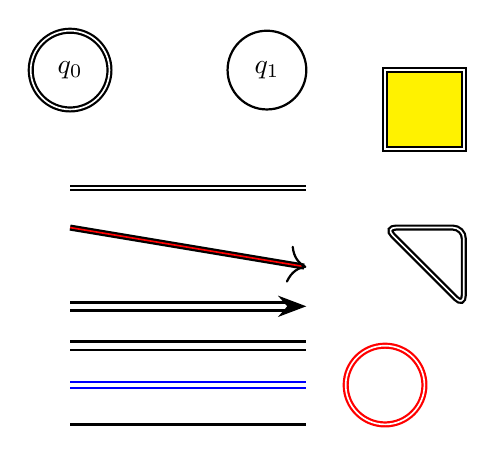
\begin{tikzpicture}[thick, state/.style={circle, draw, minimum size=1cm}]
\node[state, double] (q0) at (0,0) {$q_0$};
\node[state] (q1) at (2.5,0) {$q_1$};
\draw[double] (0,-1.5) -- (3,-1.5);
\draw[double=red, ->] (0,-2) -- (3,-2.5);
\draw[double distance=2pt, line width=1pt, -Stealth] (0,-3) -- (3,-3);
\draw[double distance between line centers=3pt] (0,-3.5) -- (3,-3.5);
\draw[double equal sign distance, blue] (0,-4) -- (3,-4);
\draw[double, double=none] (0,-4.5) -- (3,-4.5);
\draw[double, fill=yellow] (4,-1) rectangle (5,0);
\draw[double, rounded corners] (4,-2) -- (5,-2) -- (5,-3) -- cycle;
\tikzset{every double/.style={red}}
\draw[double] (4,-4) circle (0.5);
\end{tikzpicture}
\end{document}
